\documentclass[a4paper]{article}
\usepackage{color}              %Farben, f.r \definecolor{}
\usepackage{amssymb}            %Mathematische Symbole
\usepackage{amsthm}             %Besseres \newtheorem
\usepackage{amsmath}           %Mathematische Umgebungen
\usepackage{mathtools}          %\xRightarrow, etc
\usepackage{mathrsfs}           %enthaelt \mathscr
\usepackage{graphicx}
\usepackage{enumerate}          % in-place numerations def.
\usepackage{fullpage}

%Hugrún's additions
\usepackage{hyperref}
\usepackage{blkarray}

\usepackage{tikz}
\newcommand{\LD}{\langle}
\newcommand{\RD}{\rangle}
\usepackage{tikz}
\usepackage{tikz,fullpage}
\usetikzlibrary{arrows,%
                petri,%
                topaths}%
\usepackage{tkz-berge}
\usepackage[position=top]{subfig}

%------------------------

\usepackage{array}
%\usepackage{multicol}
%\usepackage[notref,notcite]{showkeys}
%\usepackage{algorithm,algorithmic}
\usepackage{color}

\usepackage{graphicx}
\usepackage{xypic}
\entrymodifiers={+!!<0pt,\fontdimen22\textfont2>}
\usepackage[all]{xy}

\newtheoremstyle{myremark} % name
    {7pt}                    % Space above
    {7pt}                    % Space below
    {}  	                 % Body font
    {}                           % Indent amount
    {\bf}       	         % Theorem head font
    {.}                          % Punctuation after theorem head
    {.5em}                       % Space after theorem head
    {}  % Theorem head spec (can be left empty, meaning ‘normal’)

\theoremstyle{plain}
\newtheorem{lemma}{Lemma}
\newtheorem{theorem}[lemma]{Theorem}
\newtheorem{fact}[lemma]{Fact}
\newtheorem{definition}[lemma]{Definition}
\newtheorem{corollary}[lemma]{Corollary}
\newtheorem{proposition}[lemma]{Proposition}
\newtheorem{conjecture}[lemma]{Conjecture}
\newtheorem{observation}[lemma]{Observation}
\newtheorem{problem}[lemma]{Problem}
\newtheorem{notation}[lemma]{Notation}
\newtheorem*{claim}{Claim}

\theoremstyle{myremark}
\newtheorem{remark}[lemma]{Remark}
\newtheorem{example}[lemma]{Example}

%%%%%% EDIT HERE: %%%%%%%%%%%
\newcommand{\LECTURENUMBER}{1A}
\newcommand{\LECTURETITLE}{Intro to Graph Theory}
\newcommand{\LECTURESCRIBE}{Hugr\'un Fj\'ola}

%% Dokument Beginn %%%%%%%%%%%%%%%%%%%%%%%%%%%%%%%%%%%%%%%%%%%%%%%%%%%%%%%%
\begin{document}
\thispagestyle{empty}

\begin{center}
	{\Large\bf Graph coloring}\\
	{\bf Lecture notes, vol. \LECTURENUMBER, \LECTURETITLE}\\
\end{center}
Lecturer: Michal Adamaszek \hfill Scribe: \LECTURESCRIBE
\begin{center}
\line(1,0){450}
\end{center}

%%%%%%% EDIT ALSO BELOW: %%%%%%%%%%%%%%%%


{\bf Formalities about the course:}
\begin{itemize}
\item There will be 3 homework assignments. Each assignment can earn you 10 points. All in all, 30 points.
\item You have the possibility to earn 3 points by volunteering to take one day of lecture notes and setting them up in LaTeX, for everyone to use. Please volunteer.
\item You will have the possibility to present an open problem, related to Graph Coloring. This will be done in the exercise sessions. Presentations should be 5-10 min.
\item There will be some computer experiments. We will use \href{https://cloud.sagemath.com/}{SageMath} (\url{https://cloud.sagemath.com/}). Please set up an account befor exercise class on Friday, 12th of February.
\item We will not be using Absalon, but you can find everything about the course on the course \href{http://www.mimuw.edu.pl/~aszek/chromatic/index.html}{website} (\url{http://www.mimuw.edu.pl/~aszek/chromatic/index.html})

\item For some literature; we will not follow a single book, at least not linearly. But Michal recommends the books by West, Bondy \& Murty or Diestel. You can find the Diestel book online (go through the course website). The others should be available in the Library.
\end{itemize}

\begin{center}
\line(1,0){450}
\end{center}

{\bf \large \noindent Introduction to Graph Theory.}
\newline

\noindent{\bf Types of Graphs:}
\begin{itemize}
    \item A (simple) graph (we will mostly look at them)\newline
    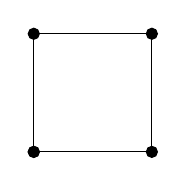
\begin{tikzpicture}
    \tikzstyle{every node}=[draw,circle,fill=black,minimum size=4pt,inner sep=0pt]
    
    \draw (0,0) node {}
        -- ++(0:1.5cm) node {}
        -- ++(90:1.5cm) node {}
        -- ++(180:1.5cm) node {}
        -- ++(270:1.5cm) node {};
\end{tikzpicture}
    \item A multi-graph\newline (multiple edges between a specific pair of vertices)
    \item A directed graph (the edges have a direction)
    \item A labelled graph (a labelled version of any other graph type. The edges have some more information)
\end{itemize}

\begin{example}
{\bf Real-world graphs. }Roadmaps, tree of game, brain, chemistry (representation of chemical compounds, Systematic IUPAC), maps, scheduling (as a \textit{matching problem} in a graph)
\end{example}

\noindent{\bf The First Problem in Graph Theory}
\newline
\indent\textit{Seven Bridges of K\"onigsberg} (now Kaliningrad, Russia)\cite{Bridges}. Euler\cite{Euler} solved this problem in 1736 and is considered to  be the first problem in Graph Theory.
\newline
The problem: \textit{Is there a tour of the city which goes through each bridge once?} No!
\newline
\underline{Why not?}
\begin{itemize}
    \item A \underline{closed} (begins and ends at the same point) walk visits each vertex an even number of times.
    \item Any walk (not necessarily closed) visits its non-endpoints an even number of times.
\end{itemize}

\begin{definition}
A simple graph is a pair $G=(V,E)$ where
\newline
$V$ is the set of vertices
\newline
$E \subseteq {V\choose 2}$, is the set of edges. (A subset of the set of all 2-element subsets of $V$)
\end{definition}

\begin{example}
A graph $G$ with vertices $V=\{a,b,c,d\}$ and edges $E=\left\{\{a,b\},\{b,c\},\{a,c\},\{c,d\}\right\}$
\end{example}

\newpage
\begin{notation}
We will be using the following notations (obs. sometimes for simplicity symbols/letters are dropped here and there, but then it should be obvious what is meant):
\begin{itemize}
    \item $xy\in E(G)$ instead of $\{x,y\}\in E(G)$
    \item $N_G(x)=\{y: xy\in E(G)\}$ is the neighborhood of $x$ in $G$. (Example above: $N(b)=\{a,c\}$)
    \item $xy\in E(G)$ we say $x,y$ are \underline{adjacent}, or \underline{neigbors} in G.
    \item a vertex is \underline{incident} to the edges that contain it.
    \item UNLESS OTHERWISE NOTED, ALL GRAPHS ARE \underline{FINITE AND SIMPLE}
\end{itemize}
\end{notation}

\begin{example}
Some key examples of families of graphs.
\begin{itemize}
    \item \underline{Cycles:} $C_n,\ n\geq 3$.\newline
    $V=\{1,\dots,n\}$\newline
    $E=\{12,23,\dots,(n-1)n,n1\}$
    \item \underline{Paths:} A subset of a cycle, $P_n,\ n\geq 1$
    \item \underline{Complete graphs:} $K_n,\ n\geq 1$\newline 
    $V=\{1,\dots,n\}$\newline
    $E={V \choose 2}$, all possible pairs of $V$\newline
    Note! $|E(K_n)|={n \choose 2}=\frac{n(n-1)}{2}$
    \item $\overline{K_n},\ n\geq 1$ (the complement of a complete graph)\newline 
    $V=\{1,\dots,n\}$\newline
    $E=\varnothing$
    \item \underline{The Empty Graph:} denoted $\varnothing$;\newline 
    $V(\varnothing)=\varnothing$\newline
    $E(\varnothing)=\varnothing$
\end{itemize}
\end{example}

\begin{definition}
The complement of $G$ is the graph $\overline{G}$ s.t.
$$
V(\overline{G})=V(G)
$$
$$
E(\overline{G})= {V(G)\choose 2}\setminus E(G)
$$
\end{definition}

\begin{example}
$Q_n,\ n\geq 1$\newline
$V(Q_n)=\{(x_1,\dots,x_n):\ x_i\in\{0,1\}\}$, all binary sequences of length $n$.\newline
$(x_1,\dots x_n)(y_1,\dots,y_n)\in E(Q_n)$ iff $(x_1,\dots x_n)(y_1,\dots,y_n)$ are different in exactly one position.\newline
\begin{itemize}
    \item $n=1$\newline
    $V(Q_1)=\{0,1\}$\newline
    $E(Q_1)=\{01\}$
    \item $n=2$\newline
    $V(Q_2)=\{00,01,10,11\}$\newline
    $E(Q_2)=\{\{00,10\},\{00,01\},\{01,11\},\{10,11\}\}$
    \item $n=3$\newline
    $V(Q_3)=\{000,001,010,100,011,101,110,111\}$\newline
    $E(Q_3)=\{\{000,001\},\{000,010\},\dots,\{011,111\}\}$
\end{itemize}
\end{example}

\begin{definition}
$G=(V,E)$. For a vertex $v\in V$, the \underline{degree} of $v,\ \deg(v)$, is the number of edges incident to $v$.
$$
\deg(v) = |N(v)|
$$
$v$ is called \underline{isolated} if $\deg(v)=0$\newline
$v$ is called \underline{a leaf} if $\deg(v)=1$
\end{definition}

\begin{lemma}
$$
\sum_{v\in V(G)}^{} \deg(v)=2\cdot|E(G)|
$$
\end{lemma}

\begin{proof}
Obvious, the sum counts every edge twice.\newline
A Very Formal Proof: Let M be a matrix of size $|V|\times |E|$
\[
    M_{v,e}= 
\begin{cases}
    1,  & \text{if $v$ is incident to $e$}\\
    0,  & \text{otherwise}
\end{cases}
\]
This is also called the incidence matrix of $G$. Let's see an example before we continue with the proof.

\begin{example}
$V=\{a,b,c,d\}$ and $E=\{ab,bc,cd\}$.
\[
M=
\begin{blockarray}{cccc}
 & ab & bc & cd \\
\begin{block}{c(ccc)}
  a & 1 & 0 & 0\\
  b & 1 & 1 & 0\\
  c & 0 & 1 & 1\\
  d & 0 & 0 & 1\\
\end{block}
\end{blockarray}
 \]
\end{example}
\noindent Now, let's continue with the proof.\newline 
The number of $1's$ in $M$ is:
\[
\begin{cases}
    2\times |E|,  & \text{(two $1's$ in each column)}\\
    \sum_{v}^{} \deg(v),  & \text{($\deg(v)\, 1's$ in $n$-th row)}
\end{cases}
\]
(this is called double counting).
\end{proof}

\begin{corollary}
The number of vertices of odd degree in every graph is even.
\end{corollary}

\begin{notation}
 $\,$
    \begin{itemize}
        \item $\Delta (G)=$ maximum vertex degree in $G$
        \item $\delta (G)=$ minimal vertex degree in $G$
        \item $G$ is called $d$-regular if $\Delta(G)=\delta(G)=d$, equivalently $\forall v\in V\, \deg(v)=d$. (Example: $Q_n$)
    \end{itemize}
\end{notation}

\noindent{\bf The Category of Graphs.}
\begin{definition}
A graph, $H$, is a subgraph of $G$ if:
\begin{itemize}
    \item $V(H)\subseteq{V(G)}$ and $E(H)\subseteq{E(G)}$. ($H$ is also a graph, so $E(H)\subseteq {{V(H) \choose 2}}$)
    \item $W \subseteq V(G)$ then \underline{$G[W]$} is the subgraph of $G$ \underline{induced by W}, which means, $$V(G[W])=W$$ $$E(G[W])=\{xy; xy\in E(G), x,y\in W\}$$

\end{itemize}
\end{definition}

\begin{example}
Induced subgraphs
\end{example}

\begin{definition}
$f:G\rightarrow H$ is a \underline{graph homomorphism} if $f:V(G)\rightarrow V(H)$, \newline s.t. $xy\in E(G)\Rightarrow f(x)f(y)\in E(H)$
\end{definition}

\begin{definition}
$G$ and $H$ are \underline{isomorphic} if $\exists\,f:G\rightarrow H$ and $g:H\rightarrow G$ s.t. $gf=1_G, fg=1_H$.
\end{definition}

\begin{observation}
$1_G:G\rightarrow G$ is homomorphism. $f:G\rightarrow H$, $g:H\rightarrow K$ are homomorphisms, then so is $gf:G\rightarrow K$.
\end{observation}

\begin{remark}
Deciding if two graphs are isomorphic is computationally hard. Proving non-isomorphism is usually about finding some invariant that distinguishes the two graphs.
\end{remark}

%%%%%%%%%%%%%%%%%%%%%%%%%%%%%%%%%%%%%%%%
\begin{thebibliography}{9}
\bibitem{Bridges} Seven Bridges of K\"onigsberg, \url{https://en.wikipedia.org/wiki/Seven_Bridges_of_K%C3%B6nigsberg}
\bibitem{Euler} Leonard Euler (1707-1783), \url{https://en.wikipedia.org/wiki/Leonhard_Euler}

\end{thebibliography}

\end{document}




